%%fakesection HEADER
\documentclass[a4paper, 10pt, onecolumn]{article} 

%-------- FONTS AND SYMBOLS-------------------------------------
\usepackage{amsmath,amssymb,bm}
\usepackage{eurosym}
\usepackage{wasysym} % some special symbol? 
\usepackage{multicol}
%\frenchspacing

\usepackage{charter}
%\usepackage[T1]{fontenc}
%\usepackage[latin1]{inputenc}
%\usepackage[scaled]{helvet}
%\renewcommand*\familydefault{\sfdefault} %% Only if the base font of the document is to be sans serif


%-------- REFERENCES -------------------------------------------
\usepackage[round,authoryear]{natbib}
%\usepackage[numbers]{natbib}
%\usepackage[super]{natbib}
\usepackage[hyperindex=true,breaklinks]{hyperref}
\hypersetup{
	colorlinks=true,
	citecolor=linkcol,
	filecolor=linkcol,
	urlcolor =linkcol,
	linkcolor=linkcol,
}
\urlstyle{same}
\usepackage{url}

%-------- INDEX ------------------------------------------------
\usepackage{makeidx}
\makeindex
\newcommand{\mytwocoltoc}{
	{\small
	\parskip 0pt
	\columnsep 24pt
	\begin{multicols}{2}
	\tableofcontents
	\end{multicols}
	\parskip 8pt
	}
}

%-------- FIGURES, CAPTIONS ETC. -------------------------------
\usepackage[dvips]{graphicx}
\usepackage[margin=20pt,labelfont=sc,indention=.5cm]{caption} 	% figure captions
\makeatletter
	\newcommand\figcaption{\def\@captype{figure}\caption}
\makeatother

\usepackage{sidecap}
\usepackage{rotating}
\usepackage{colortbl}
\usepackage[table]{xcolor}
\usepackage{tabularx}
\usepackage{booktabs}
%\usepackage[nolists]{endfloat}

\usepackage{multirow}

\newcommand{\mypic}[3]{
	\marginpar{\hspace{-#1cm}\parbox{#2\textwidth}{\includegraphics[width=#2\textwidth]{#3}}}
}

\newcommand{\mypicc}[4]{
	\marginpar{\hspace{-#1cm}\parbox{#2\textwidth}{\includegraphics[width=#2\textwidth]{#3}\\\small\raggedleft#4}}
}

\let \oldmarginpar\marginpar
\newcommand{\mymarginpar}[1]{\oldmarginpar{{\parbox{2.4cm}{\small\raggedright #1}}}}
\newcommand{\mymarginparr}[3]{\oldmarginpar{\hspace{-#1cm}{\parbox{#2cm}{\small\raggedright #3}}}}

\renewcommand{\marginpar}[1]{\-\oldmarginpar{\small\raggedright #1}}

\newcommand{\myig}[2]{\includegraphics[width=#1\textwidth]{#2}}
\newcommand{\myigg}[3]{\parbox{#1\textwidth}{\vspace{.25em}\includegraphics[width=#1\textwidth]{#2}\\\small\raggedleft#3}}

\newcommand{\mybox}[2]{\fbox{ \begin{minipage}{#1\textwidth} #2 \end{minipage}}}
\newcommand{\myboxw}[3]{\fcolorbox{white}{#2}{\begin{minipage}{#1\textwidth} #3 \end{minipage}}}
\newcommand{\sidebox}[3]{\marginpar{\hspace{-#1cm}\fbox{\begin{minipage}{#2cm} #3 \end{minipage}}}}
\newcommand{\sideboxc}[4]{\marginpar{\hspace{-#1cm}\fcolorbox{white}{#3}{\begin{minipage}{#2cm} #4 \end{minipage}}}}

\newcommand{\defin}[1]{\begin{center}\fcolorbox{red}{dyellow}{\parbox{.7\textwidth}{\centering #1}}\end{center}}
\newcommand{\nb}[1]{{\dotfill \raggedleft \small\itshape (#1)}}


%-------- PAGE LAYOUT-------------------------------------------
\usepackage{geometry}
%\textwidth=16cm \hoffset=-2cm \textheight=23cm \voffset=-1.5cm 		% a4 new
\geometry{textwidth=16cm,textheight=23cm}		% a4 new
%\newcommand{\air}{\textwidth=17cm \hoffset=-2.5cm \textheight=21.5cm \voffset=-2cm} 		% a4 on air 
\newcommand{\air}{\geometry{textwidth=17cm,textheight=21.5cm}}		% a4 new
%\textwidth=15cm \hoffset=-1.5cm \textheight=24cm \voffset=-2cm 		% a4
%\textwidth=16cm \hoffset=-2cm \textheight=22.5cm \voffset=-2.5cm 	% letter
%\textwidth=17cm \hoffset=-.7cm \textheight=24cm \voffset=-2cm 		% two columns


%-------- PARAGRAPH LOOK ---------------------------------------
\setcounter{secnumdepth}{3}	% numbering 
\setcounter{tocdepth}{2}
\parindent 0pt
\parskip 8pt
%\usepackage{setspace} 
%\doublespacing
%\onehalfspacing


%-------- HEADER -----------------------------------------------
\usepackage{fancyhdr}
\pagestyle{fancyplain}


%-------- SUPPLEMENTARY MATERIAL -------------------------------
\newcommand{\supplementarymaterial}{
	\newpage
	\section{Supplementary Material}

	\renewcommand{\thefigure}{S\arabic{figure}}
	\renewcommand{\thetable}{S\arabic{table}} 
	\renewcommand{\thesection}{S\arabic{section}}
	\renewcommand{\thesubsection}{S\arabic{subsection}}
	\renewcommand{\thesubsubsection}{S\arabic{subsubsection}}

	\setcounter{figure}{0} 
	\setcounter{table}{0}
	\setcounter{section}{0}
	\setcounter{subsubsection}{0}
}

%-------- REFERENCES -------------------------------------------
\newcommand{\myrefs}{
	\section{References}
	\renewcommand\refname{}
	\vspace{-2ex}
	\bibsep 0pt
	\bibliographystyle{apalike}
	\bibliography{../fullrefs}
}

%-------- COLOURS ----------------------------------------------

\usepackage{color}

\definecolor{blues}{rgb}{.2,.2,.5}  
\definecolor{blueds}{rgb}{0,0,.3}  
\definecolor{bluess}{rgb}{.2,.2,.8}  
\definecolor{linkcol}{rgb}{0,0,.3}  
\definecolor{red}{rgb}{.9,.1,.1}  

\newcommand{\blues}  {\textcolor{blues}}
\newcommand{\blueds}  {\textcolor{blueds}}
\newcommand{\bluess}  {\textcolor{bluess}}
\newcommand{\linkcol}  {\textcolor{linkcol}}
\newcommand{\red}  {\textcolor{red}}

\newcommand{\emb}[1]{\blueds{\bf #1}}
\newcommand{\emf}[1]{\blueds{\em #1}}
\newcommand{\emr}[1]{\red{\em #1}}



%-------- LISTS ------------------------------------------------
\usepackage{mdwlist}	 % for basedescript modified description environment

\renewcommand{\i}{\item}
\newenvironment{myit}
	{\parskip 0pt
		\begin{itemize*} 
		\setlength{\itemsep}{0pt} 
		\setlength{\parskip}{0pt} 
		\setlength{\parsep}{0pt}
		\setlength{\topsep}{-8pt}
	}
	{\parskip 6pt \end{itemize*}}

\newenvironment{myenum}
	{\parskip 0pt
		\begin{enumerate*} 
		\setlength{\itemsep}{0pt} 
		\setlength{\parskip}{0pt} 
		\setlength{\parsep}{0pt}
		\setlength{\topsep}{-8pt}
	}
	{\parskip 8pt \end{enumerate*}}

\newenvironment{myde}
	{\parskip 0pt
	\begin{basedescript}{\desclabelstyle{\pushlabel} \desclabelwidth{2.5em}}
		\renewcommand{\makelabel}[1]{\blueds{\bf##1}\hfil}
		\setlength{\itemsep}{0pt} 
		\setlength{\parskip}{0pt} 
		\setlength{\parsep}{0pt}
		\setlength{\topsep}{0pt}
	}
	{\end{basedescript} \parskip 8pt}



%-------- SECTIONS ETC. ----------------------------------------

\usepackage{ifthen}

% \@startsection {NAME}{LEVEL}{INDENT}{BEFORESKIP}{AFTERSKIP}{STYLE} 
%            optional * [ALTHEADING]{HEADING}
%    Generic command to start a section.  
%    NAME       : e.g., 'subsection'
%    LEVEL      : a number, denoting depth of section -- e.g., chapter=1,
%                 section = 2, etc.  A section number will be printed if
%                 and only if LEVEL < or = the value of the secnumdepth
%                 counter.
%    INDENT     : Indentation of heading from left margin
%    BEFORESKIP : Absolute value = skip to leave above the heading.  
%                 If negative, then paragraph indent of text following 
%                 heading is suppressed.
%    AFTERSKIP  : if positive, then skip to leave below heading,
%                       else - skip to leave to right of run-in heading.
%    STYLE      : commands to set style
%  If '*' missing, then increments the counter.  If it is present, then
%  there should be no [ALTHEADING] argument.  A sectioning command
%  is normally defined to \@startsection + its first six arguments.


\makeatletter
\def\section      {\@startsection{section}{1}{1pt}{-3.5ex plus -1ex minus -.2ex}{1.5ex plus .2ex}{\sc\Large\blues}}
\def\subsection   {\@startsection{subsection}   {2}{0pt}{-2.25ex plus -1ex minus -.2ex}{1.0ex plus .2ex}{\large\sc\bluess}}
\def\subsubsection{\@startsection{subsubsection}{3}{0pt}{-0.25ex plus -.2ex minus -.1ex}{0.2ex plus .05ex}{\normalsize\it\bluess}}
\makeatother



\graphicspath{ {./figs/} }
\newcommand{\ra}{\ensuremath{\rightarrow}\/ }
\newcommand{\la}{\ensuremath{\leftarrow}\/ }

\newcommand{\ts}[1]{\textsuperscript{#1}}

\DeclareMathOperator*{\argmax}{argmax}
\DeclareMathOperator*{\argmin}{argmin}

\newcommand{\TT}{\ensuremath^{\text{T}}}
\newcommand{\tth}{\ensuremath^{\text{\tiny th}}}
\newcommand{\inv}{\ensuremath^{-1}}
\newcommand{\dd}[2]{\frac{d #1}{d #2}}
\newcommand{\D}[2]{\frac{\partial #1}{\partial #2}}
\newcommand{\DD}[2]{\frac{\partial ^2 #1}{\partial #2 ^2}}
\newcommand{\Di}[2]{\frac{\partial ^i #1}{\partial #2 ^i}}
\newcommand{\bic}{BIC$_{\mathsf{int}}$\/ }

\newcommand{\bfa}{\ensuremath\mathbf{a}}
\newcommand{\bfb}{\ensuremath\mathbf{b}}
\newcommand{\bfc}{\ensuremath\mathbf{c}}
\newcommand{\bfd}{\ensuremath\mathbf{d}}
\newcommand{\bfe}{\ensuremath\mathbf{e}}
\newcommand{\bff}{\ensuremath\mathbf{f}}
\newcommand{\bfg}{\ensuremath\mathbf{g}}
\newcommand{\bfh}{\ensuremath\mathbf{h}}
\newcommand{\bfi}{\ensuremath\mathbf{i}}
\newcommand{\bfj}{\ensuremath\mathbf{j}}
\newcommand{\bfk}{\ensuremath\mathbf{k}}
\newcommand{\bfl}{\ensuremath\mathbf{l}}
\newcommand{\bfm}{\ensuremath\mathbf{m}}
\newcommand{\bfn}{\ensuremath\mathbf{n}}
\newcommand{\bfo}{\ensuremath\mathbf{o}}
\newcommand{\bfp}{\ensuremath\mathbf{p}}
\newcommand{\bfq}{\ensuremath\mathbf{q}}
\newcommand{\bfr}{\ensuremath\mathbf{r}}
\newcommand{\bfs}{\ensuremath\mathbf{s}}
\newcommand{\bft}{\ensuremath\mathbf{t}}
\newcommand{\bfu}{\ensuremath\mathbf{u}}
\newcommand{\bfv}{\ensuremath\mathbf{v}}
\newcommand{\bfw}{\ensuremath\mathbf{w}}
\newcommand{\bfx}{\ensuremath\mathbf{x}}
\newcommand{\bfy}{\ensuremath\mathbf{y}}
\newcommand{\bfz}{\ensuremath\mathbf{z}}

\newcommand{\bfA}{\ensuremath\mathbf{A}}
\newcommand{\bfB}{\ensuremath\mathbf{B}}
\newcommand{\bfC}{\ensuremath\mathbf{C}}
\newcommand{\bfD}{\ensuremath\mathbf{D}}
\newcommand{\bfE}{\ensuremath\mathbf{E}}
\newcommand{\bfF}{\ensuremath\mathbf{F}}
\newcommand{\bfG}{\ensuremath\mathbf{G}}
\newcommand{\bfH}{\ensuremath\mathbf{H}}
\newcommand{\bfI}{\ensuremath\mathbf{I}}
\newcommand{\bfJ}{\ensuremath\mathbf{J}}
\newcommand{\bfK}{\ensuremath\mathbf{K}}
\newcommand{\bfL}{\ensuremath\mathbf{L}}
\newcommand{\bfM}{\ensuremath\mathbf{M}}
\newcommand{\bfN}{\ensuremath\mathbf{N}}
\newcommand{\bfO}{\ensuremath\mathbf{O}}
\newcommand{\bfP}{\ensuremath\mathbf{P}}
\newcommand{\bfQ}{\ensuremath\mathbf{Q}}
\newcommand{\bfR}{\ensuremath\mathbf{R}}
\newcommand{\bfS}{\ensuremath\mathbf{S}}
\newcommand{\bfT}{\ensuremath\mathbf{T}}
\newcommand{\bfU}{\ensuremath\mathbf{U}}
\newcommand{\bfV}{\ensuremath\mathbf{V}}
\newcommand{\bfW}{\ensuremath\mathbf{W}}
\newcommand{\bfX}{\ensuremath\mathbf{X}}
\newcommand{\bfY}{\ensuremath\mathbf{Y}}
\newcommand{\bfZ}{\ensuremath\mathbf{Z}}

\newcommand{\mbbA}{\ensuremath\mathbb{A}}
\newcommand{\mbbB}{\ensuremath\mathbb{B}}
\newcommand{\mbbC}{\ensuremath\mathbb{C}}
\newcommand{\mbbD}{\ensuremath\mathbb{D}}
\newcommand{\mbbE}{\ensuremath\mathbb{E}}
\newcommand{\mbbF}{\ensuremath\mathbb{F}}
\newcommand{\mbbG}{\ensuremath\mathbb{G}}
\newcommand{\mbbH}{\ensuremath\mathbb{H}}
\newcommand{\mbbI}{\ensuremath\mathbb{I}}
\newcommand{\mbbJ}{\ensuremath\mathbb{J}}
\newcommand{\mbbK}{\ensuremath\mathbb{K}}
\newcommand{\mbbL}{\ensuremath\mathbb{L}}
\newcommand{\mbbM}{\ensuremath\mathbb{M}}
\newcommand{\mbbN}{\ensuremath\mathbb{N}}
\newcommand{\mbbO}{\ensuremath\mathbb{O}}
\newcommand{\mbbP}{\ensuremath\mathbb{P}}
\newcommand{\mbbQ}{\ensuremath\mathbb{Q}}
\newcommand{\mbbR}{\ensuremath\mathbb{R}}
\newcommand{\mbbS}{\ensuremath\mathbb{S}}
\newcommand{\mbbT}{\ensuremath\mathbb{T}}
\newcommand{\mbbU}{\ensuremath\mathbb{U}}
\newcommand{\mbbV}{\ensuremath\mathbb{V}}
\newcommand{\mbbW}{\ensuremath\mathbb{W}}
\newcommand{\mbbX}{\ensuremath\mathbb{X}}
\newcommand{\mbbY}{\ensuremath\mathbb{Y}}
\newcommand{\mbbZ}{\ensuremath\mathbb{Z}}

\newcommand{\mca}{\ensuremath\mathcal{A}}
\newcommand{\mcb}{\ensuremath\mathcal{B}}
\newcommand{\mcc}{\ensuremath\mathcal{C}}
\newcommand{\mcd}{\ensuremath\mathcal{D}}
\newcommand{\mce}{\ensuremath\mathcal{E}}
\newcommand{\mcf}{\ensuremath\mathcal{F}}
\newcommand{\mcg}{\ensuremath\mathcal{G}}
\newcommand{\mch}{\ensuremath\mathcal{H}}
\newcommand{\mci}{\ensuremath\mathcal{I}}
\newcommand{\mcj}{\ensuremath\mathcal{J}}
\newcommand{\mck}{\ensuremath\mathcal{K}}
\newcommand{\mcl}{\ensuremath\mathcal{L}}
\newcommand{\mcm}{\ensuremath\mathcal{M}}
\newcommand{\mcn}{\ensuremath\mathcal{N}}
\newcommand{\mco}{\ensuremath\mathcal{O}}
\newcommand{\mcp}{\ensuremath\mathcal{P}}
\newcommand{\mcq}{\ensuremath\mathcal{Q}}
\newcommand{\mcr}{\ensuremath\mathcal{R}}
\newcommand{\mcs}{\ensuremath\mathcal{S}}
\newcommand{\mct}{\ensuremath\mathcal{T}}
\newcommand{\mcu}{\ensuremath\mathcal{U}}
\newcommand{\mcv}{\ensuremath\mathcal{V}}
\newcommand{\mcw}{\ensuremath\mathcal{W}}
\newcommand{\mcx}{\ensuremath\mathcal{X}}
\newcommand{\mcy}{\ensuremath\mathcal{Y}}
\newcommand{\mcz}{\ensuremath\mathcal{Z}}


\pagestyle{fancy}
\renewcommand{\sectionmark}[1]{\markboth{#1}{ }}
\rhead{\sc{\leftmark}}
\lfoot{\sc{}}
\rfoot{\sc{Not for circulation}}

\newcommand{\ts}[1]{\textsuperscript{#1}}

\begin{document}

\newcommand{\shorttitle}{Power analysis}
\renewcommand{\title}{Power analysis for efficacy RCT based on pilot safety RCT\par}
\thispagestyle{empty}

{\huge \title }

{\bf Quentin J.M. Huys
}

When doing power analyses, we try to estimate how large the sample has to be so
that, after running the study, we have a certain degree of certainty that if an
effect of a certain size was there we didn't miss it. The effect size the size
of the difference between the groups, and does not refer to whether this size of
difference is significant. An effect of size d may be visible in a small study,
but not statistically significant. So significance and effect size are different
measures. 

When planning a study, we ask how large the sample needs to be so that for an
effect of a given size we are likely to observe a significant effect with some
probability. This probability is the power. It is standard for efficacy trials
to aim for a power of 90\%, i.e. for a probability of 90\% that a group
comparison will be significant, given that in truth there was a group difference
of a certain assumed size d. 

The effect size and hence power estimates obviously depend a lot on whether we
do an ITT or PP analysis: they are much larger in the PP than the ITT analyses,
because of course ITT includes people who did not do the therapy really. 

We ran a safety RCT comparing waitlist to the intervention component of the app
alone. 50 participants were randomized to each group. We'd now like to estimate
the size of the new efficacy RCT based on these results. The results are shown
in figure~\ref{f:power}. The top row shows the curves for all participants (ITT,
left), only those who did the therapy (PP, middle), and then also the analysis
when subtracting baseline SPIN scores in the PP analysis. The effects are
weakest in ITT, as one would expect. In this sample, the effects are stronger
when looking at change scores (right). 

The bottom row of plots in figure~\ref{f:power} shows the power for different
sample sizes, when basing the effect size on the respective
definitions/analyses. The dashed red line shows the 90\% power, so that
determines the sample size we should shoot for. 

As we want to make statements about the app as a whole, it may make sense for
the primary analysis to be on an ITT sample. This would measure overall
improvement in the two groups independent of whether participants actually
engaged in the app itself. But it means that the result is very meaningful as it
also captures how much people do want to engage with the app, which will e
important for how well it does in reality. 

Judging from the pilot RCT, the ITT effect size at week 4 is between 0.2 and
0.34 (see top left panel). Basic power analyses and simulations suggest that we
would need a sample of around 250 for this. I would suggest this is what we aim
for. 

\begin{sidewaysfigure}[htbp]
\begin{center}
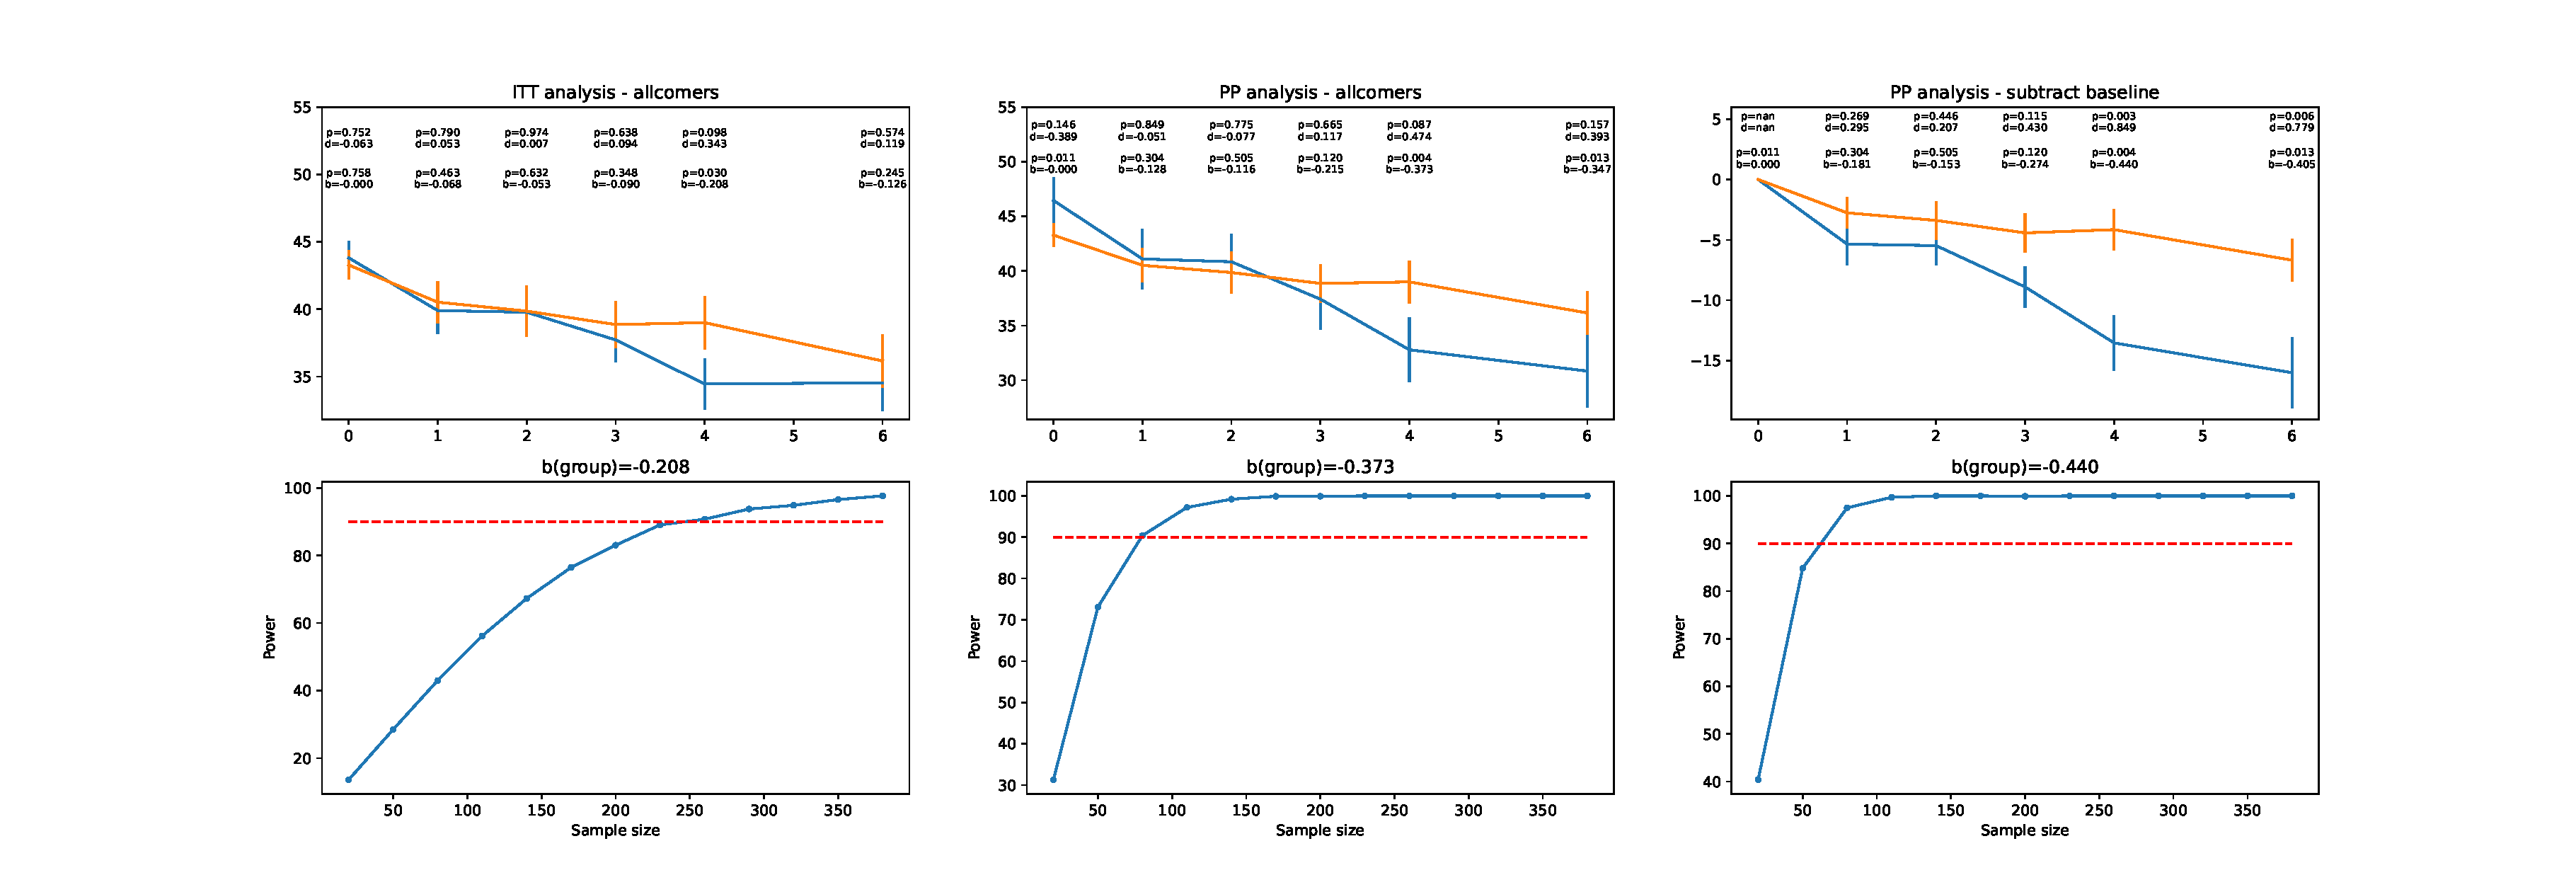
\includegraphics[width=\textwidth]{RCT_poweranalysis.pdf}
\end{center}
\caption{Analysis of RCT data. Orange is waitlist, blue intervention. The top
row shows SPIN scores and analyses, the bottom row power analyses. 
%
{\bf Top left}: ITT analysis. The top row of statistics shows simple t-tests and Cohen's d for each
week. The bottom row shows standardized $\beta$ estimates for the group effect
for a linear regression with baseline spin, age and group, with the dependent
variable being the spin score at each of the weeks. 
%
{\bf Bottom left}: Power analysis for ITT analysis. I extracted the week 4 beta
values from the regression (bottom line of results in the panel above), and
simulated this, counting the number of times a significant result was achieved.
A simple power analysis for a 2-sample t-test for a Cohen's d of 0.343 yiels an
$N=294$. Repeating this but using as effect size the standardized regression
coefficient of 0.208 yields an $N=794$. The simulate power analysis suggests a
total sample size of $N=250$. 
%
{\bf Top middle}: PP analysis. This only includes participants who were marked
as 'completers'. The top row of statistics again shows simple t-tests and Cohen's d for each
week. The bottom row shows standardized $\beta$ estimates for the group effect
for a linear regression with baseline spin, age and group, with the dependent
variable being the spin score at each of the weeks. 
%
{\bf Bottom middle}: Power analysis for PP analysis. I extracted the week 4 beta
values from the regression (bottom line of results in the panel above), and
simulated this, counting the number of times a significant result was achieved.
This suggests a total sample size of $N=90$. 
A simple power analysis for a 2-sample t-test for a Cohen's d of 0.474 yields an
$N=154$. Repeating this but using as effect size the standardized regression
coefficient of 0.373 yields an $N=248$. 
%
{\bf Top right}: PP analysis on difference scores. This only includes participants who were marked
as 'completers'. Baseline values were subtracted from subsequent values, so this
is an analysis of difference scores from baseline. 
The top row of statistics again shows simple t-tests and Cohen's d for each
week. The bottom row shows standardized $\beta$ estimates for the group effect
for a linear regression with baseline spin, age and group, with the dependent
variable being the spin score at each of the weeks. 
%
%
{\bf Bottom right}: Power analysis for PP analysis on difference scores. I extracted the week 4 beta
values from the regression (bottom line of results in the panel above), and
simulated this, counting the number of times a significant result was achieved.
This suggests a total sample size of $N=76$. 
A simple power analysis for a 2-sample t-test for a Cohen's d of 0.849 yields an
$N=50$. Repeating this but using as effect size the standardized regression
coefficient of 0.440 yields an $N=180$. 
}
\label{f:power}
\end{sidewaysfigure}






\end{document}


